% 2p5d-two-die-heatsink: heat-flow network with an EXPLICIT heatsink node (TikZ).
% Source: config/thermal/2p5d-two-die-heatsink-explicit.yaml (schema v1.1).
% Compile: pdflatex 2p5d-two-die-heatsink.tex   (TeX Live 2026)
%
% v3.2 (author): the heatsink is a modeling dimension, not a boundary.
% Heat path (fully orthogonal): die0/die1 ->(tim, conduction R=0.3 K/W)->
% heatsink node (free node, its own cooling resistance R_conv) ->
% (heatsink_ambient, convection R=1/(hA)=0.69 K/W)-> ambient. Every branch
% is annotated with its physical path type and the value's provenance
% (geometry + material from the config YAML).
%
% Edge styling: face_adjacency = solid blue; tim/heatsink_ambient =
% solid amber arrows. All routing orthogonal (no diagonals).
\documentclass[border=10pt]{standalone}
\usepackage{sfmath}
\renewcommand{\familydefault}{\sfdefault}
\usepackage{tikz}
\usetikzlibrary{arrows.meta, shapes.geometric}
\definecolor{diefill}{HTML}{E8F0FE}   % die: light blue fill
\definecolor{dieedge}{HTML}{1A73E8}
\definecolor{hsfill}{HTML}{E0F2F1}    % heatsink: teal rounded rectangle
\definecolor{hsedge}{HTML}{00695C}
\definecolor{bndfill}{HTML}{F1F3F4}   % boundary: light gray ellipse
\definecolor{bndedge}{HTML}{5F6368}
\definecolor{faedge}{HTML}{1A73E8}    % face_adjacency: solid blue
\definecolor{vcedge}{HTML}{B45309}    % vertical_chain: solid amber arrow
\begin{document}
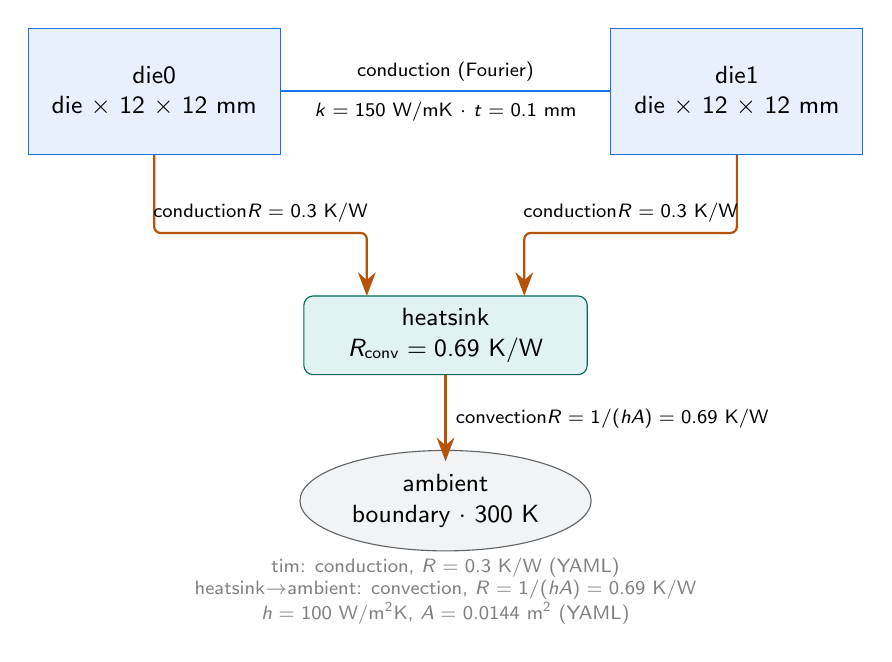
\begin{tikzpicture}[
  die/.style={rectangle, draw=dieedge, fill=diefill, minimum width=3.2cm,
              minimum height=1.6cm, align=center, font=\small},
  hs/.style={rectangle, rounded corners=0.12cm, draw=hsedge, fill=hsfill,
             minimum width=3.6cm, minimum height=1.0cm, align=center, font=\small},
  bnd/.style={ellipse, draw=bndedge, fill=bndfill, minimum width=3.0cm,
              minimum height=1.1cm, align=center, font=\small},
  fa/.style={draw=faedge, thick},
  vc/.style={draw=vcedge, thick, -{Stealth[length=3mm]}, rounded corners=0.08cm},
  lab/.style={font=\scriptsize},
]
\node[die] (die0) at (-3.7,  1.6) {die0\\die $\times$ 12 $\times$ 12 mm};
\node[die] (die1) at ( 3.7,  1.6) {die1\\die $\times$ 12 $\times$ 12 mm};
\node[hs]   (hs)   at ( 0.0, -1.5) {heatsink\\$R_{\mathrm{conv}}=0.69$ K/W};
\node[bnd]  (ambient) at (0, -3.6) {ambient\\boundary $\cdot$ 300 K};
\draw[fa] (die0.east) -- node[above, lab] {conduction (Fourier)}
                      node[below, lab] {$k=150$ W/mK $\cdot$ $t=0.1$ mm} (die1.west);
% vertical chains: die ->(TIM, conduction)-> heatsink ->(convection)-> ambient
\draw[vc] (die0.south) -- (-3.7,-0.2) -- node[above, lab] {conduction\\$R=0.3$ K/W} (-1.0,-0.2) -- (-1.0,-1.0);
\draw[vc] (die1.south) -- ( 3.7,-0.2) -- node[above, lab] {conduction\\$R=0.3$ K/W} ( 1.0,-0.2) -- ( 1.0,-1.0);
\draw[vc] (hs.south) -- node[right, lab] {convection\\$R=1/(hA)=0.69$ K/W} (0, -3.10);
% branch annotation: physical path type + value provenance (geometry+material)
\node[lab, align=center, text=gray] at (0, -4.75) {
  tim: conduction, $R=0.3$ K/W (YAML)\\
  heatsink$\rightarrow$ambient: convection, $R=1/(hA)=0.69$ K/W\\
  $h=100$ W/m$^2$K, $A=0.0144$ m$^2$ (YAML)};
\end{tikzpicture}
\end{document}
